\section{Results}


Each assessment was done with the following target coordinates.

\begingroup
{\centering
    \begin{tabular}{|l|l|l|l|l|l|}
    \hline
    \textbf{Target} & \textbf{1} & \textbf{2} & \textbf{3} & \textbf{4} & \textbf{5}  \\ \hline
    \textbf{x}      & 0.35       & -0.35      & 0.5        & -0.35      & 0.35        \\ \hline
    \textbf{y}      & 0.3        & 0.4        & -0.4       & 0          & 0.4         \\ \hline
    \end{tabular}
    \begin{tabular}{|l|l|l|l|l|l|}
        \hline
        \textbf{Target} & \textbf{6} & \textbf{7} & \textbf{8} & \textbf{9} & \textbf{10} \\ \hline
        \textbf{x}      & -0.15      & -0.35      & 0.35       & -0.5       & 0.35        \\ \hline
        \textbf{y}      & -0.1       & -0.3       & -0.4       & 0.4        & 0           \\ \hline
        \end{tabular}
}
\endgroup


Each simulation was also run for 3000 simulation steps and 5000 epochs.

In this simulation, the heuristic algorithm hit 5 targets and achieved a value for the sum of rewards as 4894.42, against our chosen reward function.

The following graph shows an example of the Soft state Monti-Carlo state machine algorithm’s results, under the same conditions. \Cref{fig:fig1}.

We modelled the cumulative reward function for any given epoch using the least-squares optimized log function. \Cref{fig:fig1}. The implementation is not deterministic therefore an average of five simulations is used to reduce the error in our least squares exponential model.
\\
The Logarithmic line for best fit is defined by the following equation:

\begingroup\centering
$1475.01044*ln(0.00310817391CumuliveReward) + 1642.65857$
\endgroup

The model has a residual standard deviation of 711.29847146. 

Figure 2 shows targets hit against cumulative rewards.

\begin{figure}
    \centering
    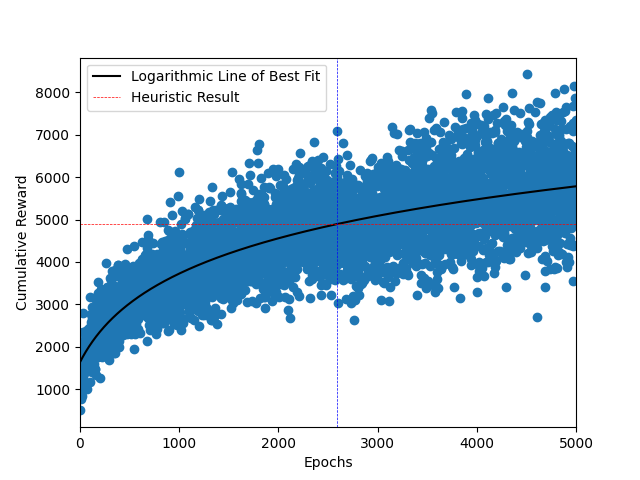
\includegraphics[width=\singlefigure]{figures/figure_2.png}
    \caption{\label{fig:fig1} Shows Logarithmic line of best fit of the data with result of the heuristic.}
\end{figure}

\begin{figure}
    \centering
    \includegraphics[width=\singlefigure]{figures/figure_3.png}
    \caption{\label{fig:fig2} Shows correlation between how many targets hit and cumulative reward for simulation.}
\end{figure}